\documentclass[11pt,a4paper]{article}

\usepackage[utf8]{inputenc}
\usepackage[T1]{fontenc}
\usepackage[brazil]{babel}
\usepackage{lmodern}
\usepackage[a4paper,margin=2.3cm]{geometry}
\usepackage{amsmath,amssymb,amsthm}
\usepackage{graphicx}
\usepackage{booktabs}
\usepackage{float}
\usepackage{caption}
\usepackage{subcaption}
\usepackage{xcolor}
\usepackage[hidelinks]{hyperref}

\captionsetup{font=small,labelfont=bf}
\setlength{\parskip}{0.4em}
\setlength{\emergencystretch}{2em}

\newtheorem{lema}{Lema}
\newcommand{\preencher}[1]{\textcolor{red}{\textbf{[#1]}}}
\newcommand{\Oh}{\mathcal{O}}

\title{\textbf{Divisão e Conquista:\\ Subarranjo de Soma Máxima e Par de Pontos Mais Próximos}}
\author{Francisco Magno \and Guilherme Azevedo\\[0.4em]
\small Projeto e Análise de Algoritmos, Universidade de Fortaleza (UNIFOR)}
\date{Novembro de 2026}

\begin{document}
\maketitle

\begin{abstract}
Implementamos dois problemas resolvidos por divisão e conquista, o subarranjo de soma máxima e o par de pontos mais próximos, cada um acompanhado de uma solução de força bruta, e acrescentamos o algoritmo de Kadane, em $\Theta(n)$, para o primeiro problema. As recorrências foram resolvidas analiticamente e os tempos de execução foram medidos para entradas de 10 a 6.400 elementos. Os resultados confirmam o crescimento previsto pela análise: a divisão e conquista passa a superar a força bruta a partir de $n = {100}$ na Etapa~1 e de $n = {25}$ na Etapa~2, e o limiar mais rápido para o caso base da Etapa~2 foi ${8}$. O código, os testes e as medições brutas estão disponíveis em  \url{https://github.com/GuilhermeMAzevedo/divisao-e-conquista}.
\end{abstract}

\section{Metodologia}

Os algoritmos foram implementados em Python. Cada versão recebe a entrada como lista e devolve o resultado, sem leitura ou escrita dentro do algoritmo, o que permite testá-las e medi-las da mesma forma. As medições foram feitas pelo script \texttt{medicao.py} na máquina descrita na Tabela~\ref{tab:maquina}.

\begin{table}[H]
\centering\small
\begin{tabular}{ll}
\toprule
Processador & {Intel Core i5-14600KF (14ª geração), 3.50 GHz} \\
Memória RAM & {16,0 GB DDR4, 2666 MHz} \\
Sistema operacional & {Windows 11 Pro, versão 26H2} \\
Python & {CPython 3.15.0} \\
\bottomrule
\end{tabular}
\caption{Configuração da máquina usada nas medições.}
\label{tab:maquina}
\end{table}

Usamos os tamanhos $n \in \{10, 25, 50, 100, 200, 400, 800, 1600, 3200, 6400\}$. Os tamanhos de 100 a 6.400 são os pedidos no enunciado; os menores foram incluídos para localizar o ponto em que a força bruta deixa de ser mais rápida. Para cada tamanho fizemos 5 repetições, e as tabelas mostram a média e o desvio padrão. Alguns cuidados foram tomados para que as medições fossem comparáveis:

\begin{itemize}
  \item em cada tamanho e repetição, todos os algoritmos de uma etapa recebem exatamente a mesma entrada, gerada com semente fixa;
  \item a geração da entrada fica fora do tempo medido, cronometrado com \texttt{time.perf\_counter};
  \item o coletor de lixo do Python é desligado durante cada medição, para não interromper uma execução no meio;
  \item cada algoritmo roda uma vez antes das medições, sem ser cronometrado, como aquecimento.
\end{itemize}

Na Etapa~1, os vetores têm inteiros uniformes em $[-100, 100]$. Na Etapa~2, os pontos têm coordenadas reais uniformes em $[0, 10^6]$. As medições brutas, uma linha por execução, estão nos arquivos \texttt{resultados.csv} e \texttt{resultados\_limiar.csv} do repositório.

\section{Etapa 1: Subarranjo de Soma Máxima}

Dado um vetor $A[0..n-1]$ de inteiros, que representa a variação diária do preço de uma ação, queremos o intervalo contínuo $A[i..j]$ de maior soma. A saída é a soma e os índices $i$ e $j$, contados a partir de 0. Quando vários intervalos têm a mesma soma máxima, adotamos a seguinte \textbf{regra de desempate}: vence o que começa mais cedo e, persistindo o empate, o que termina mais cedo. As três versões seguem a mesma regra, o que permite comparar suas respostas diretamente nos testes.

\subsection{Força bruta}

Para cada início $i$, a soma é acumulada enquanto o fim $j$ avança, de modo que cada intervalo custa $\Theta(1)$. O número de intervalos testados é
\[
\sum_{i=0}^{n-1} (n - i) = \frac{n(n+1)}{2} = \Theta(n^2).
\]

\subsection{Divisão e conquista}

O vetor é dividido ao meio, em $m = \lfloor (\ell + r)/2 \rfloor$, e o melhor intervalo é o maior entre três candidatos: o melhor inteiramente na metade esquerda, o melhor inteiramente na metade direita, ambos obtidos recursivamente, e o melhor que cruza o meio. Este último contém obrigatoriamente $A[m]$ e $A[m+1]$, e pode ser calculado em $\Theta(n)$ com duas varreduras independentes: uma de $m$ para a esquerda, que acha o melhor início, e outra de $m+1$ para a direita, que acha o melhor fim. Como as duas escolhas são independentes, a soma das melhores partes é a melhor soma que cruza o meio.

Para respeitar a regra de desempate, a varredura para a esquerda atualiza o início também em caso de igualdade ($\geq$), ficando com o início mais cedo, e a varredura para a direita só atualiza com melhora estrita ($>$), ficando com o fim mais cedo. Na combinação, os três candidatos são comparados pela chave (soma, $-$início, $-$fim). Não basta preferir a metade esquerda em caso de empate, porque um intervalo que cruza o meio pode começar antes do melhor intervalo da metade esquerda.

\paragraph{Recorrência.} O caso base ($n = 1$) custa $\Theta(1)$, e cada nível faz duas chamadas de metade do tamanho mais um trabalho linear:
\[
T(n) = 2\,T(n/2) + \Theta(n).
\]
Pelo Teorema Mestre~\cite{clrs}, com $a = 2$ e $b = 2$, temos $n^{\log_b a} = n$ e $f(n) = \Theta(n) = \Theta(n^{\log_b a})$, o que corresponde ao caso~2 e dá $T(n) = \Theta(n \log n)$. A árvore de recursão confirma o resultado: o nível $k$ tem $2^k$ subproblemas de tamanho $n/2^k$, com custo total $cn$ por nível, e há $\log_2 n + 1$ níveis, totalizando $cn\log_2 n + cn = \Theta(n \log n)$.

\subsection{Versão linear: algoritmo de Kadane}

O algoritmo de Kadane~\cite{bentley} percorre o vetor uma vez, mantendo a maior soma de um intervalo que termina na posição atual. Ao avançar para $A[j]$, a soma acumulada só é descartada, recomeçando em $j$, quando ela é negativa; quando é exatamente zero, estender o intervalo mantém a soma e preserva o início mais cedo, de acordo com a regra de desempate. Como cada elemento é processado uma única vez em tempo constante, o custo é $\Theta(n)$.

\subsection{Resultados}

A Tabela~\ref{tab:etapa1} e a Figura~\ref{fig:etapa1} mostram os tempos medidos.

\begin{table}[H]
\centering\small
\begin{tabular}{rrrr}
\toprule
$n$ & Força bruta & Divisão e conquista & Kadane \\
\midrule
10 & 0,006 $\pm$ 0,003 & 0,017 $\pm$ 0,005 & 0,003 $\pm$ 0,002 \\
25 & 0,012 $\pm$ 0,002 & 0,040 $\pm$ 0,010 & 0,005 $\pm$ 0,002 \\
50 & 0,027 $\pm$ 0,001 & 0,046 $\pm$ 0,003 & 0,005 $\pm$ 0,001 \\
100 & 0,091 $\pm$ 0,002 & 0,080 $\pm$ 0,002 & 0,006 $\pm$ 0,001 \\
200 & 0,320 $\pm$ 0,026 & 0,174 $\pm$ 0,041 & 0,009 $\pm$ 0,001 \\
400 & 1,415 $\pm$ 0,302 & 0,355 $\pm$ 0,118 & 0,015 $\pm$ 0,001 \\
800 & 6,092 $\pm$ 1,638 & 0,648 $\pm$ 0,081 & 0,027 $\pm$ 0,006 \\
1600 & 26,335 $\pm$ 2,247 & 1,385 $\pm$ 0,203 & 0,047 $\pm$ 0,001 \\
3200 & 103,991 $\pm$ 2,693 & 2,800 $\pm$ 0,161 & 0,093 $\pm$ 0,002 \\
6400 & 432,887 $\pm$ 4,539 & 5,648 $\pm$ 0,089 & 0,183 $\pm$ 0,006 \\
\bottomrule
\end{tabular}

\caption{Etapa 1: tempo médio $\pm$ desvio padrão, em milissegundos, em 5 execuções.}
\label{tab:etapa1}
\end{table}

\begin{figure}[H]
\centering
\begin{subfigure}{0.49\textwidth}
  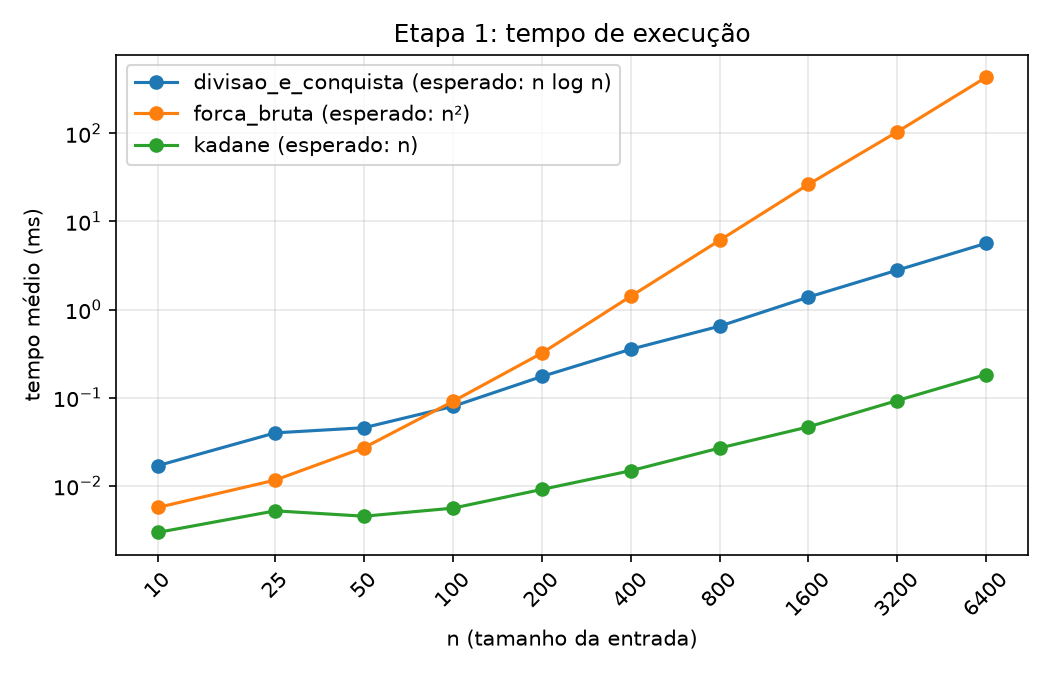
\includegraphics[width=\linewidth]{graficos/etapa1_tempo.png}
  \caption{Tempo médio em escala log-log.}
\end{subfigure}\hfill
\begin{subfigure}{0.49\textwidth}
  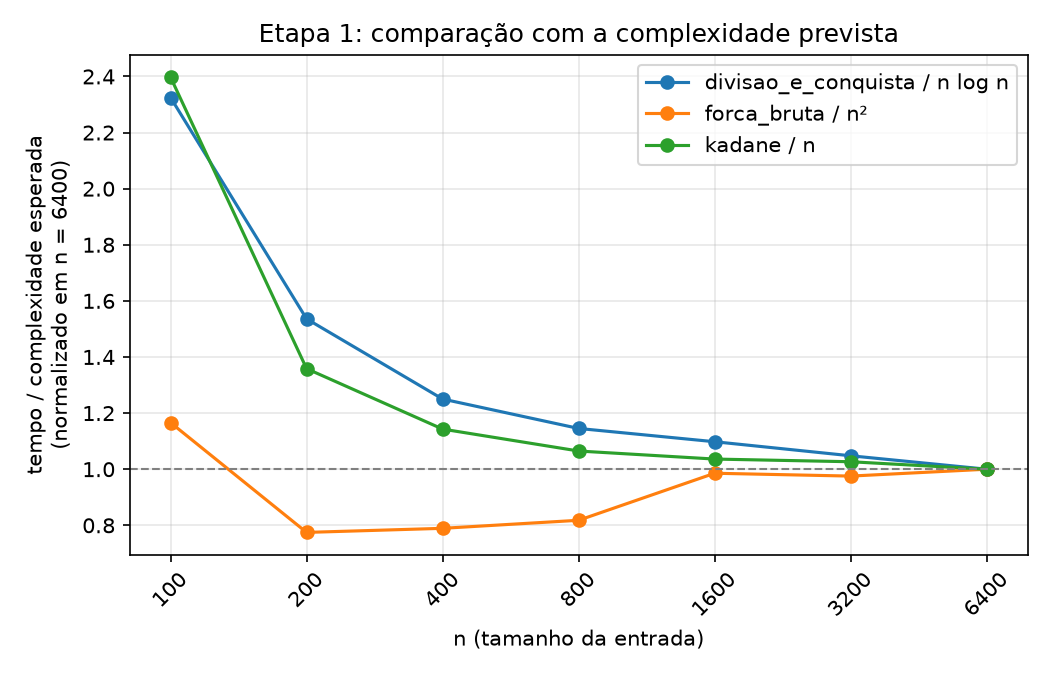
\includegraphics[width=\linewidth]{graficos/etapa1_razao.png}
  \caption{Tempo dividido pela complexidade prevista.}
\end{subfigure}
\caption{Etapa 1: comportamento observado e previsto.}
\label{fig:etapa1}
\end{figure}

Em escala log-log, uma função $cn^k$ aparece como uma reta de inclinação $k$. Assim, esperamos inclinação próxima de 2 para a força bruta, ligeiramente acima de 1 para a divisão e conquista e igual a 1 para Kadane. {Ao dobrar $n$ de 3200 para 6400, o tempo da força bruta foi multiplicado por 4,16 (o esperado para $n^2$ é 4), o da divisão e conquista por 2,02 (cerca de 2,17 para $n\log n$) e o de Kadane por 1,97 (2 para $n$). A força bruta foi mais rápida até $n = 50$ (0,027~ms contra 0,046~ms), e a divisão e conquista passou a vencer a partir de $n = 100$, em todos os tamanhos seguintes. Em $n = 6400$, a diferença já é de 432,9~ms contra 5,6~ms.}

O gráfico (b) divide o tempo médio pela complexidade prevista ($n^2$, $n\log n$ ou $n$), normalizando pelo valor em $n = 6400$. Se a análise estiver correta, a curva se aproxima de 1 conforme $n$ cresce. {As três curvas se aproximam de 1 a partir de $n \approx 1600$, o que indica que, nessa faixa, o tempo cresce na proporção prevista. Para $n$ menores, a divisão e conquista e Kadane ficam acima de 1 (1,73 e 2,10 em $n = 100$), porque os custos fixos de cada execução, como chamadas de função e criação de listas, pesam mais quando há pouco trabalho a fazer. A força bruta faz o contrário e fica um pouco abaixo de 1 para $n$ pequeno (entre 0,76 e 0,90). Não investigamos a causa; uma possibilidade é o cache de inteiros pequenos do Python, que mantém prontos os valores de $-5$ a 256: com vetores maiores, as somas acumuladas saem mais vezes dessa faixa e exigem criar novos objetos, o que encarece cada operação.}

\section{Etapa 2: Par de Pontos Mais Próximos}

Dadas as coordenadas de $n \geq 2$ estações em um plano, queremos as duas mais próximas segundo a distância euclidiana. A força bruta compara todos os $\binom{n}{2} = \Theta(n^2)$ pares. Quando vários pares têm a mesma distância mínima, qualquer um deles é uma resposta correta; por isso, os testes comparam a distância e verificam se o par devolvido de fato tem essa distância.

\subsection{Divisão e conquista}

Seguimos o algoritmo clássico~\cite{clrs,kt}. Os pontos são ordenados por $x$ uma única vez, antes da recursão. Cada chamada então:

\begin{enumerate}
  \item \textbf{divide} os pontos pela posição na lista ordenada (a mediana), e não pelo valor de $x$, o que mantém a divisão equilibrada mesmo quando vários pontos têm o mesmo $x$;
  \item \textbf{resolve} cada metade recursivamente, obtendo a menor distância $\delta$ entre as duas;
  \item \textbf{combina} intercalando as listas das duas metades, já ordenadas por $y$, como no \emph{merge sort}, seleciona os pontos da faixa $|x - x_m| < \delta$ em torno da linha divisória $x = x_m$ e compara cada ponto da faixa com no máximo os 7 seguintes na ordem por $y$.
\end{enumerate}

Devolver cada metade já ordenada por $y$ evita reordenar a faixa em toda chamada, o que custaria $\Theta(n\log n)$ por nível e levaria o total a $\Theta(n\log^2 n)$.

\paragraph{Recorrência.} A intercalação, a seleção da faixa e a varredura com no máximo 7 comparações por ponto custam $\Theta(n)$ cada:
\[
T(n) = 2\,T(n/2) + \Theta(n) = \Theta(n\log n),
\]
pelo mesmo raciocínio da Etapa~1. Somando a ordenação inicial, também $\Theta(n\log n)$, o custo total é $\Theta(n\log n)$.

\subsection{Por que bastam 7 comparações por ponto}

\begin{lema}
Seja $\delta$ a menor distância encontrada nas duas metades. Se dois pontos $p$ e $q$ da faixa estão a uma distância menor que $\delta$, então, na lista da faixa ordenada por $y$, $q$ está no máximo 7 posições depois de $p$ (supondo $p$ antes de $q$).
\end{lema}

\begin{proof}
Seja $y_p \leq y_q$. Como $d(p,q) < \delta$, temos $y_q < y_p + \delta$. Todo ponto que aparece entre $p$ e $q$ na lista ordenada tem $y$ entre $y_p$ e $y_q$ e está na faixa, portanto pertence ao retângulo
\[
R = [x_m - \delta,\, x_m + \delta] \times [y_p,\, y_p + \delta],
\]
de largura $2\delta$ e altura $\delta$. Basta então mostrar que $R$ contém no máximo 8 pontos.

Divida $R$ em 8 quadrados de lado $\delta/2$: quatro com $x \in [x_m - \delta, x_m]$, que associamos à metade esquerda, e quatro com $x \in [x_m, x_m + \delta]$, que associamos à metade direita. Cada ponto da metade esquerda que está em $R$ cai em um quadrado esquerdo, e cada ponto da metade direita, em um quadrado direito.

Dois pontos da mesma metade estão a uma distância de pelo menos $\delta$, pois $\delta$ é a menor distância dentro de cada metade. Já a maior distância possível dentro de um quadrado é a sua diagonal, $\delta/\sqrt{2} < \delta$. Logo, cada quadrado contém no máximo um ponto da metade a que está associado, e $R$ contém no máximo $4 + 4 = 8$ pontos. Descontando o próprio $p$, restam no máximo 7, e $q$ está entre eles.
\end{proof}

Na implementação, a varredura também para antes das 7 comparações quando a diferença em $y$ atinge $\delta$, pois nenhum ponto seguinte pode estar mais perto. Além disso, $\delta$ diminui sempre que um par mais próximo é encontrado na faixa, o que só torna a busca mais restrita.

\subsection{Escolha do limiar}

Abaixo de um certo tamanho, comparar todos os pares é mais rápido do que continuar dividindo, porque cada nível da recursão tem custos fixos: chamadas de função, cópias de listas e a intercalação. Com um limiar $k$ (subproblemas com até $k$ pontos são resolvidos por força bruta), há cerca de $n/k$ casos base de custo $\Theta(k^2)$ e $\log_2(n/k)$ níveis de combinação, logo
\[
T(n) = \Theta\!\left(\frac{n}{k}\cdot k^2 + n\log\frac{n}{k}\right) = \Theta\!\left(nk + n\log\frac{n}{k}\right).
\]
Para $k$ constante, a complexidade continua $\Theta(n\log n)$; o limiar só altera as constantes. Um $k$ pequeno demais aumenta o número de chamadas recursivas, e um $k$ grande demais faz o termo quadrático dos casos base dominar. O melhor valor, portanto, é determinado experimentalmente.

Medimos a divisão e conquista com $n = 6400$ e limiares de 2 a 64 (Tabela~\ref{tab:limiar} e Figura~\ref{fig:limiar}).

\begin{figure}[H]
\centering
\begin{minipage}{0.36\textwidth}
  \centering\small
  \begin{tabular}{rr}
\toprule
Limiar & Tempo médio (ms) \\
\midrule
2 & 13,285 $\pm$ 0,159 \\
3 & 17,242 $\pm$ 6,200 \\
4 & 11,934 $\pm$ 0,669 \\
8 & \textbf{10,948 $\pm$ 0,220} \\
16 & 12,005 $\pm$ 0,384 \\
32 & 16,001 $\pm$ 0,375 \\
64 & 25,201 $\pm$ 0,585 \\
\bottomrule
\end{tabular}

  \captionof{table}{Tempo da D\&C com $n = 6400$ para cada limiar (ms).}
  \label{tab:limiar}
\end{minipage}\hfill
\begin{minipage}{0.6\textwidth}
  \centering
  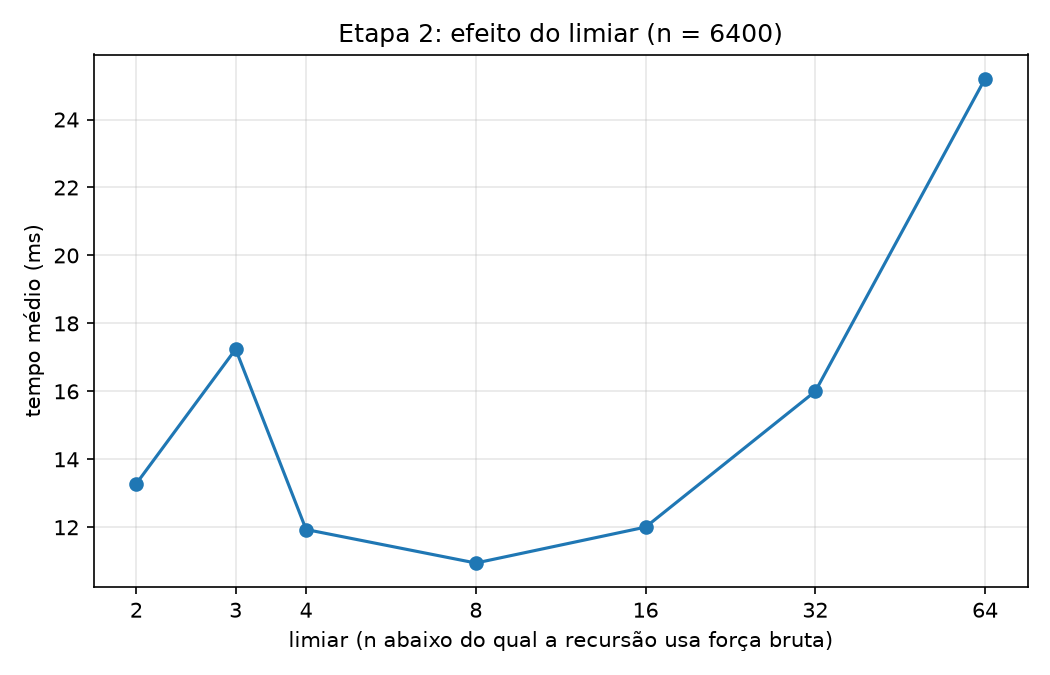
\includegraphics[width=\linewidth]{graficos/etapa2_limiar.png}
  \caption{Efeito do limiar no tempo da divisão e conquista.}
  \label{fig:limiar}
\end{minipage}
\end{figure}

{A Tabela~\ref{tab:limiar} mostra que o limiar 8 foi o mais rápido. Limiares menores, como 2 e 3, levam a recursão até subproblemas muito pequenos, e o custo fixo dessas chamadas extras supera o que se economiza em comparações. Limiares grandes, como 32 e 64, voltam a piorar porque cada caso base faz $\Theta(k^2)$ comparações, e esse termo passa a dominar. Entre esses extremos, os dois efeitos se equilibram.} Por isso, adotamos limiar ${8}$ na implementação final, e é com ele que foram feitas as medições da Tabela~\ref{tab:etapa2}.

\subsection{Resultados}

\begin{table}[H]
\centering\small
\begin{tabular}{rrr}
\toprule
$n$ & Força bruta & Divisão e conquista \\
\midrule
10 & 0,011 $\pm$ 0,003 & 0,015 $\pm$ 0,003 \\
25 & 0,044 $\pm$ 0,001 & 0,031 $\pm$ 0,001 \\
50 & 0,169 $\pm$ 0,007 & 0,079 $\pm$ 0,030 \\
100 & 0,647 $\pm$ 0,039 & 0,150 $\pm$ 0,058 \\
200 & 2,695 $\pm$ 0,190 & 0,269 $\pm$ 0,026 \\
400 & 10,240 $\pm$ 0,129 & 0,541 $\pm$ 0,017 \\
800 & 41,188 $\pm$ 0,362 & 1,171 $\pm$ 0,085 \\
1600 & 168,371 $\pm$ 1,174 & 2,378 $\pm$ 0,025 \\
3200 & 668,282 $\pm$ 2,026 & 5,161 $\pm$ 0,147 \\
6400 & 2688,786 $\pm$ 9,990 & 11,060 $\pm$ 0,421 \\
\bottomrule
\end{tabular}

\caption{Etapa 2: tempo médio $\pm$ desvio padrão, em milissegundos, em 5 execuções.}
\label{tab:etapa2}
\end{table}

\begin{figure}[H]
\centering
\begin{subfigure}{0.49\textwidth}
  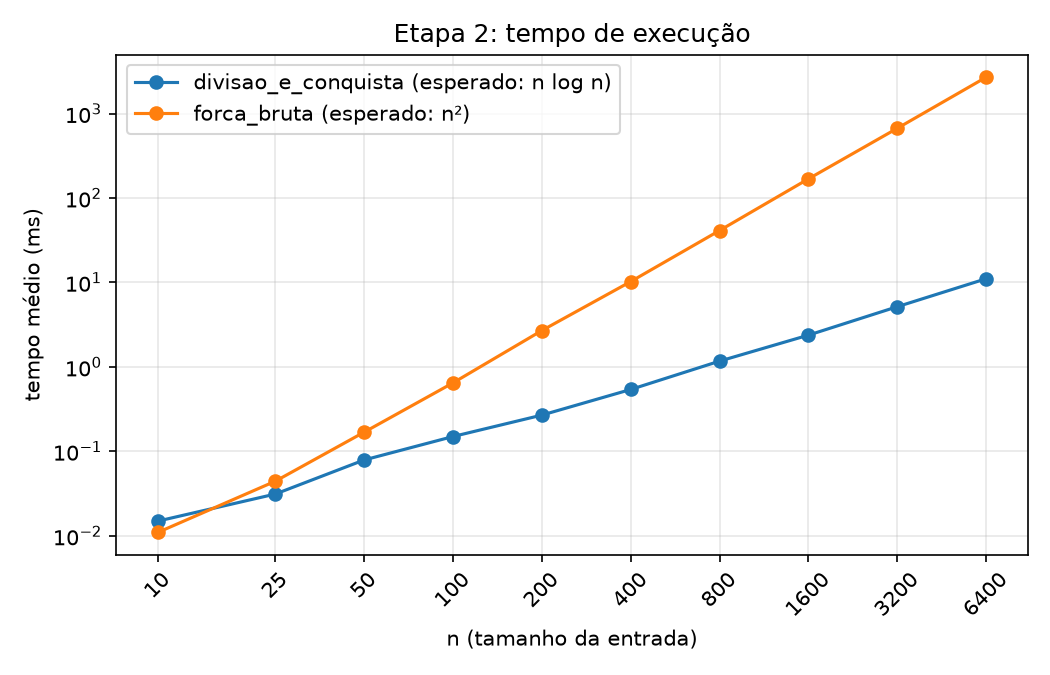
\includegraphics[width=\linewidth]{graficos/etapa2_tempo.png}
  \caption{Tempo médio em escala log-log.}
\end{subfigure}\hfill
\begin{subfigure}{0.49\textwidth}
  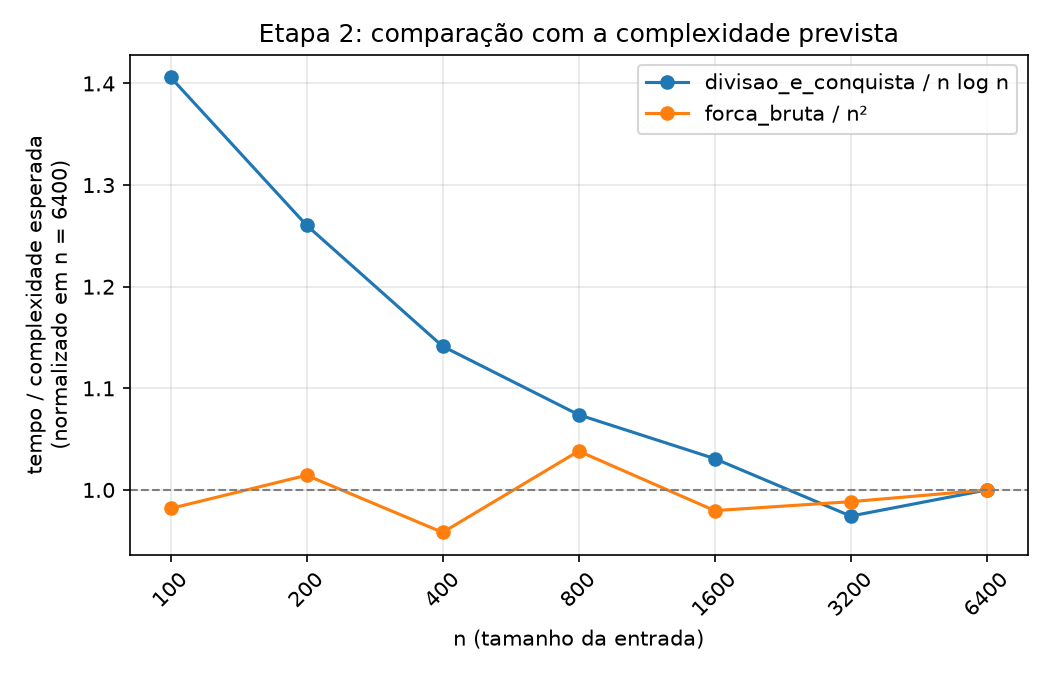
\includegraphics[width=\linewidth]{graficos/etapa2_razao.png}
  \caption{Tempo dividido pela complexidade prevista.}
\end{subfigure}
\caption{Etapa 2: comportamento observado e previsto.}
\label{fig:etapa2}
\end{figure}

{Ao dobrar $n$ de 3200 para 6400, o tempo da força bruta foi multiplicado por 4,02 e o da divisão e conquista por 2,14, muito perto dos valores esperados para $n^2$ e $n\log n$ (4 e 2,17). No gráfico~(b), a curva da força bruta fica entre 0,97 e 1,03 em toda a faixa medida, e a da divisão e conquista se aproxima de 1 a partir de $n \approx 1600$. A força bruta só foi mais rápida em $n = 10$; a partir de $n = 25$, a divisão e conquista venceu em todos os tamanhos e, em $n = 6400$, foi cerca de 243 vezes mais rápida (11,1~ms contra 2688,8~ms).}

\section{Testes}

A bateria de testes, executada com \texttt{python -m unittest discover -s testes}, tem quatro camadas:

\begin{enumerate}
  \item \textbf{Casos fixos com justificativa.} Os arquivos de casos de teste (15 casos em \nolinkurl{casos_etapa1.txt} e 13 em \nolinkurl{casos_etapa2.txt}) registram, para cada um, a entrada, a saída esperada e o motivo de existir. Eles cobrem os casos exigidos (vetor só de negativos, vetor de tamanho 1 e empates) e outros, como todos os valores nulos, máximo cruzando o meio, pontos duplicados, todos os pontos com o mesmo $x$ e par cruzando a linha divisória.
  \item \textbf{Testes diferenciais.} Milhares de entradas aleatórias pequenas são resolvidas por todas as versões, que precisam concordar. Usamos valores em intervalos estreitos, como inteiros entre $-3$ e $3$ ou coordenadas inteiras de 0 a 10, para provocar empates e pontos repetidos com frequência. Na Etapa~2, o teste também roda a D\&C com vários limiares, já que o limiar deve mudar só o tempo, nunca a resposta.
  \item \textbf{Propriedades conhecidas.} Em vetores só de negativos, a resposta é o maior elemento na primeira ocorrência; em vetores só de positivos, é o vetor inteiro. Esses testes não dependem da força bruta.
  \item \textbf{Linha de comando.} Os programas são executados como o professor fará, com a entrada em uma ou em várias linhas, incluindo entradas inválidas.
\end{enumerate}

Para avaliar a capacidade da bateria de encontrar erros, introduzimos defeitos de propósito no código (\emph{teste de mutação}) e verificamos se algum teste falhava (Tabela~\ref{tab:mutacao}).

\begin{table}[H]
\centering\small
\begin{tabular}{p{0.55\textwidth}l}
\toprule
Defeito introduzido & Detectado por \\
\midrule
Etapa 1: trocar $\geq$ por $>$ na varredura para a esquerda & apenas os testes diferenciais \\
Etapa 2: comparar só 1 vizinho na faixa, em vez de 7 & casos fixos e diferenciais \\
Etapa 2: deslocar a linha divisória & casos fixos e diferenciais \\
Etapa 2: intercalar as metades por $x$ em vez de $y$ & casos fixos e diferenciais \\
\bottomrule
\end{tabular}
\caption{Teste de mutação: defeitos introduzidos e os testes que os detectaram.}
\label{tab:mutacao}
\end{table}

O primeiro defeito altera apenas a escolha entre intervalos empatados e passou por todos os casos fixos, mas foi detectado pelos testes diferenciais. Isso mostra que as duas abordagens se complementam: os casos fixos documentam situações conhecidas, e os aleatórios encontram combinações que não prevíamos.

\section{Discussão: quando cada abordagem vence}

A análise assintótica diz como o custo cresce, mas não qual algoritmo é mais rápido para um $n$ específico, porque ignora as constantes. Para $n$ pequeno, a força bruta foi mais rápida nas duas etapas: seus laços fazem pouco trabalho por iteração e não têm custo de recursão, enquanto a divisão e conquista paga, em cada chamada, a chamada de função, a criação de listas e a combinação. Em Python esses custos fixos são especialmente altos, o que desloca o ponto de virada para a direita. Conforme $n$ cresce, a diferença entre $n^2$ e $n\log n$ supera qualquer diferença de constantes: {em $n = 6400$, a D\&C foi cerca de 77 vezes mais rápida na Etapa~1 e 243 vezes na Etapa~2}.

{O ponto de virada foi menor na Etapa~2 ($n = 25$) do que na Etapa~1 ($n = 100$). Cada comparação da força bruta da Etapa~2 calcula uma distância, com subtrações, quadrados e uma raiz quadrada, enquanto a da Etapa~1 faz só uma soma e uma comparação. Com um custo maior por iteração, o termo quadrático pesa mais cedo, e a divisão e conquista compensa já em entradas menores; pelo mesmo motivo, sua vantagem em $n = 6400$ é maior na Etapa~2. Algumas medições de tamanho intermediário tiveram desvio padrão alto em relação à média, como a força bruta da Etapa~1 em $n = 800$ (6,09~$\pm$~1,64~ms) e a divisão e conquista da Etapa~2 em $n = 100$ (0,150~$\pm$~0,058~ms). Tempos tão curtos ficam mais sensíveis a interrupções do sistema operacional e de outros programas; em $n = 6400$, o desvio ficou abaixo de 4\% da média em todos os algoritmos.}

Na Etapa~1, o algoritmo de Kadane foi o mais rápido em todos os tamanhos medidos, por combinar crescimento linear com um laço simples. A divisão e conquista, embora assintoticamente pior que Kadane, ilustra bem a técnica e serve de base para problemas em que não há solução linear conhecida.

\section{Conclusão}

As medições confirmaram as complexidades previstas pelas recorrências: ao dobrar o tamanho da entrada, o tempo das forças brutas foi multiplicado por cerca de 4, o das versões de divisão e conquista por pouco mais de 2 e o de Kadane por 2, como esperado para $\Theta(n^2)$, $\Theta(n\log n)$ e $\Theta(n)$. A força bruta só vence para entradas pequenas, abaixo de $n = 100$ na Etapa~1 e de $n = 25$ na Etapa~2, o que justifica usar um limiar no caso base: na Etapa~2, o limiar 8 foi o mais rápido entre os valores testados. Para entradas grandes, a vantagem da divisão e conquista é expressiva: em $n = 6400$, ela foi cerca de 77 vezes mais rápida que a força bruta na Etapa~1 e 243 vezes na Etapa~2. A bateria de testes, com casos de borda justificados, testes diferenciais e teste de mutação, deu confiança na correção das implementações, inclusive nos empates.

\begin{thebibliography}{9}
\bibitem{clrs}
T.~H. Cormen, C.~E. Leiserson, R.~L. Rivest e C.~Stein.
\emph{Algoritmos: teoria e prática}. 3.~ed. Rio de Janeiro: Elsevier, 2012.

\bibitem{kt}
J.~Kleinberg e É.~Tardos.
\emph{Algorithm Design}. Boston: Pearson, 2006.

\bibitem{bentley}
J.~Bentley.
\emph{Programming Pearls}. 2.~ed. Reading: Addison-Wesley, 2000.
\end{thebibliography}

\end{document}